\section{Compact Muon Solenoid Experiment} \label{section:higgs_cms}

\subsection{Large Hadron Collider} \label{subsection:higgs_cms_lhc}
\begin{figure}[hbp]
    \centering
    \subfigure[]{
        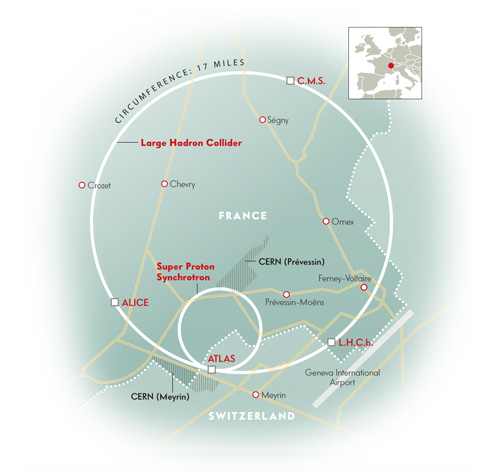
\includegraphics[width=0.99\textwidth]{figures/ch_higgs/misc/lhcring.jpg}
    }
    \caption{LHC Accelerator Complex}
    \label{fig:higgs_cms_lhc}
 \end{figure}

 The Large Hadron Collider is the particle accelerating and colliding complex located on the border between France and Switzerland. Physically speaking, it is a ring that is about 27 km in circumference and serves four major High Energy Physics Experiments: CMS, Atlas, Alice and LHCb.

\subsection{General Description} \label{subsection:higgs_cms_generaldescription}
The Compact Muon Solenoid is a two-fold creature; first of all, it is, a one of its kind, general purpose particle detector system, which consists of multiple components (to be discussed futher) and whose primary objective is to record and reconstruct physics events that could help us study the fundamental building blocks of nature. It acts like a camera, recording the footprint of the physics interactions which particle physicists use to deduce the underlying physics. The Compact Muon Solenoid is also an experiment, a collaboration of thousands of people whose combined effort made it possible to build such a device. From people involved in data-taking at Point 5 and detector maintainance experts to people performing the analysis of recorded events and making sure that the data we have collected is of the highest quality - it is one of the best examples when group effort produces results of highest estime.

The most important component of CMS that makes it stand out among other experiments is the superconducting solenoid with magnetic field of 3.8 T. The magnet is located just outside of HCAL subsystem and plays a crucial role in the overall architecture of CMS. In particular, due to the strength of magnetic field, significant improvements are expected in the search for the Higgs Boson decaying via two muons due to a high resolution of the muon system together with the power of the magnet. The closest subsystem of CMS to the interaction point is the Silicon Tracker, whose primary objective is to measure the trajectory of the charged particles passsing through. What follows are Electromagnetic and Hadronic subsystems which respectively consist of several subdetectors with varying performance characteristics. Muon Systems are located just outside of the magnet and comprise different technologies depending on the $\eta$ location.

The Large Hadron Collider is not just a challenging project from an engineering standpoint, it is also a data factory, one of its kind, that presents a unique challenge for the data processing and analysis domain. The amount of data that gets generated quickly becomes unmanagable and one has to be careful when selecting what to preserve and what to abandon. The collsion rate is about 40 MHz and the compressed size of just 1 event coming from CMS is on order of 1 KB. That amounts to 40 GB/s and if we extrapolate up to a single hour of datataking we get about 140 TB/h - obviously this becomes unfeasible very quickly. For the purpose of selection of events of interest, all HEP Experiments employ a sophisticated Trigger System, whose purpose is to select the physics events of interest. CMS has two layers of data reduction: Level 1 and High Level Trigger. Level 1 trigger system is a hardware based processing system, that is tightly integrated with the rest of the subsystems' electronics. Level 1 allows CMS to reduce the event rate from 40 MHz down to 100 KHz. This is achieved by applying basic selections at hardware level (integration with the subsystems' electronics results in zero copy processing) using reduced content information known as Trigger Primitives (TPs).

The 100 KHz output of Hardware Trigger System gets further reduced by High Level Trigger (HLC) down to 100 Hz that gets actually written to disk. This content reduction is achieved by employing high level information produced via the reconstruction procedure. Basically, CMS High Level Trigger System is a reasonable-sized High Perfomance Cluster (HPC) Complex which takes the output of Level 1 and acts as a filtering system, flagging events that should be stored to disk for offline processing. The software framework that gets used is the same one as for offline data analysis, however certain reconstruction steps are optimized for performance.

%\subsection{Tracker System} \label{subsection:higgs_cms_tracker}
%Explain Pixels and Tracker

%\subsection{Electromagnetic Calorimeter} \label{subsection:higgs_cms_em}
%Electromagnetic Calorimeter (or Ecal for breivity) is a subsystem of CMS with the primary objective to

%\subsection{Hadronic Calorimeter} \label{subsection:higgs_cms_hcal}
%Hadron Calorimeter (or Hcal for breivity) is a subsystem of CMS with the primary objective to identify and measure energy of jets. It consists of four separate parts: Hadron Barrel, Hadron Endcap, Hadron Outer and Hadron Forward.

%\subsection{Muon System} \label{subsection:higgs_cms_muon}
%Describe the Muon Systems

%\subsection{Trigger System} \label{subsection:higgs_cms_trigger}

%\subsection{Data Acquisition Software}

%\subsection{Data Analysis Software} \label{subsection:higgs_cms_cmssw}
%Describe the Software for Analysis